\documentclass[a4paper]{article}
\usepackage{fancyhdr}
\usepackage{physics}
\usepackage{graphicx}

\usepackage{subcaption}
\usepackage{floatrow}

\graphicspath{ {img/} }

\title{Meine Antwort zum erweiterten Wigner's Freund Gedankenexperiment}
\author{Jannis Naske}

\pagestyle{fancy}
\fancyhf{}
\rhead{Jannis Naske}

\pagenumbering{arabic}

\begin{document}
\maketitle

\section*{Abstract}
In diesem Dokument schlage ich zwei mögliche Korrekturen zum erweiterten Wigner's Freund Gedankenexperiment von Renner und Frauchiger vor.
Durch diese Verbesserungen wird der Widerspruch vernichtet, und alle drei Annahmen, \textbf{(Q)}, \textbf{(C)} und \textbf{(S)}, bleiben unverletzt.

\section*{Der erste Fehler}
Im Artikel von Renner und Frauchiger wird folgendes Statement hergeleitet:
\begin{itemize}
	\item \textbf{Statement 1 by} $F_1$: ``If I get $t$, I know that $W_2$ will measure $plus$''
\end{itemize}
Der Beweis, welcher benutzt wird, ist folgender(ich lasse in diesem Dokument die doppelten Symbole weg, da dies in diesem Fall redundante Information ist):\\\\
Nachdem $F_1$ $t$ gemessen hat, setzt er den Spin für $F_2$ in die Superposition $\frac{1}{\sqrt{2}} \ket{\downarrow} + \frac{1}{\sqrt{2}} \ket{\uparrow}$.
In der Basis $\qty{\ket{+}_{L_2}, \ket{-}_{L_2}}$, mit $\ket{+}_{L_2} = \frac{1}{\sqrt{2}} \ket{\downarrow} + \frac{1}{\sqrt{2}} \ket{\uparrow}$, $\ket{-}_{L_2} = \frac{1}{\sqrt{2}} \ket{\downarrow} - \frac{1}{\sqrt{2}} \ket{\uparrow}$,
ist diese Superposition dargestellt als $\ket{+}_{L_2}$, und $W_2$ wird somit $\ket{+}_{L_2}$ messen, und die Aussage folgt.\\\\
Jedoch wurde bei diesem Beweis weggelassen, dass die Superposition durch das Messen von $W_1$ verändert wird.
Wenn $W_1$ nach Annahme $\ket{-}_{L_1} = \frac{1}{\sqrt{2}}\ket{h} + \frac{1}{\sqrt{2}}\ket{t}$ misst, geht die Superposition, nach dem Artikel,
in $\ket{-}_{L_1}\ket{\uparrow} = \frac{1}{\sqrt{2}}\ket{h}\ket{\uparrow} - \frac{1}{\sqrt{2}}\ket{t}\ket{\uparrow} = \qty(\frac{1}{\sqrt{2}} \ket{h} - \frac{1}{\sqrt{2}} \ket{t})\qty(\ket{+}_{L_2} - \ket{-}_{L_2}) = \frac{1}{2}\ket{h}\ket{+}_{L_2} - \frac{1}{2}\ket{t}\ket{+}_{L_2} - \frac{1}{2}\ket{h}\ket{-}_{L_2} + \frac{1}{2}\ket{t}\ket{-}_{L_2}$ über. Es ist also doch möglich, dass $W_2$ $\ket{t}\ket{-}_{L_2}$ misst, und Statement 1 stellt sich als falsch heraus.\\\\
Zum Schluss misst $W_2$ nach Annahme noch $\ket{-}_{L_2}$, und der Zustand geht in $\frac{1}{\sqrt{2}}\ket{t}\ket{-} - \frac{1}{\sqrt{2}}\ket{h}\ket{-} = \frac{1}{2}\ket{t}\ket{\downarrow} - \frac{1}{2}\ket{t}\ket{\uparrow} - \frac{1}{2}\ket{h}\ket{\downarrow} + \frac{1}{2}\ket{h}\ket{\uparrow}$ über.

\section*{Der zweite Fehler}
Da das Statement 1 nicht mehr gilt, verschwindet die sich widersprechende Aussage aus dem ursprünglichen Bericht. Jedoch gibt es noch ein Problem. Oben haben wir den Zustand $\frac{1}{2}\ket{t}\ket{\downarrow} - \frac{1}{2}\ket{t}\ket{\uparrow} - \frac{1}{2}\ket{h}\ket{\downarrow} + \frac{1}{2}\ket{h}\ket{\uparrow}$ als Schlusszustand hergeleitet, worauf die Korrektur des ersten Fehlers keinen Einfluss hat. Wenn aber in diesem Zustand in den Standardbasen gemessen wird, ist es möglich, den Zustand $\ket{h}\ket{\uparrow}$ zu messen. Dies scheint aber aus der Perspektive von $F_1$ nicht möglich zu sein; Wenn er $\ket{h}$ misst, wird er das Qubit, dass er dann an $F_2$ weiterleitet, in den Zustand $\ket{\downarrow}$ versetzen. Ist dies ein anderer Widerspruch? Um diese Frage zu beantworten, betrachten wir zuerst ein simpleres Problem, und wenden dann unsere Erkenntnis auf das Ursprüngliche Problem an.\\\\
Der Aufbau des Experiments ist in Bild 1.1 dargestellt. $Q_1$ und $Q_2$ stellen Quantenbits dar, der Freund, $F$, befindet sich mit den Bits in einer Isolation, die dann von Wigner, $W$, gemessen wird. $Q_1$ kann die Zustände $\ket{t}$, $\ket{h}$ annehmen, und $Q_2$ $\ket{\downarrow}$, $\ket{\uparrow}$. Eine Umrandung um Elemente bedeutet, dass die Umrandung isoliert ist, der Inhalt sich also in eine Superposition versetzen lässt. Die Ellipse um $Q_1$ verdeutlicht hierbei, dass $Q_1$ von $F$ gemessen wird. Es werden die gleichen Messregeln wie im originalen Artikel angewendet. Der Plan läuft wie folgt ab:
\begin{itemize}
	\item \textbf{Schritt 1:} $F$ setzt $Q_1$ in eine Superposition $\frac{1}{\sqrt{2}} \ket{h} + \frac{1}{\sqrt{2}} \ket{t}$.
	\item \textbf{Schritt 2:} $F$ misst $Q_1$. Ist das Ergebnis $\ket{h}$, setzt er $Q_2$ als $\ket{\downarrow}$, sonst setzt er $Q_2$ als $\ket{\uparrow}$.
	\item \textbf{Schritt 3:} $W$ misst sein Labor in der Basis $\qty{\ket{+}, \ket{-}}$, mit $\ket{+} = \frac{1}{\sqrt{2}} \ket{h} + \frac{1}{\sqrt{2}} \ket{t}$ und $\ket{-} = \frac{1}{\sqrt{2}} \ket{h} - \frac{1}{\sqrt{2}} \ket{t}$.
\end{itemize}
Nach Schritt 2 hat das Labor von $W$ den Zustand $\frac{1}{\sqrt{2}} \ket{h}\ket{\downarrow} + \frac{1}{\sqrt{2}} \ket{t}\ket{\uparrow} = \frac{1}{2}\ket{+}\ket{\downarrow} + \frac{1}{2}\ket{-}\ket{\downarrow} + \frac{1}{2}\ket{+}\ket{\uparrow} - \frac{1}{2}\ket{-}\ket{\uparrow}$. Wir nehmen nun an dass $W$ $\ket{-}$ misst. Der Endzustand lautet: $\frac{1}{\sqrt{2}} \ket{-}\ket{\downarrow} - \frac{1}{\sqrt{2}} \ket{-}\ket{\uparrow} = \frac{1}{2}\ket{h}\ket{\downarrow} - \frac{1}{2}\ket{t}\ket{\downarrow} - \frac{1}{2}\ket{h}\ket{\uparrow} + \frac{1}{2}\ket{t}\ket{\uparrow}$. Auch hier sehen wir, dass aus Sicht von $F$ die Werte $\ket{t}\ket{\downarrow}$ und $\ket{h}\ket{\uparrow}$ nicht in Frage kommen. Wie kann es aber sein, dass unsere Berechnungen zu so einer Wahrscheinlichkeitsverteilung führen? Meine Behauptung: Die Annahmen, die wir bei der Berechnung beim Messen machen, sind falsch. Wir betrachten bei unserer Annahme ein Quantenregister mit zwei Qubits, im Zustand $\frac{1}{\sqrt{2}} \ket{h}\ket{\downarrow} + \frac{1}{\sqrt{2}} \ket{t}\ket{\uparrow}$, siehe Bild 1.2. $W$ misst hier das Quantenregister, welches in einer Superposition ist. Dieses Modell entspricht aber nicht der wirklichen Situation! Im richtigen Modell haben wir ein geschachteltes System: $Q_2$ ist ein Qubit im Labor von $F$, welches im Labor von $W$ ist(wobei $Q_2$ nicht unbedingt isoliert sein muss, da es nicht in eine Superposition gesetzt wird; Hier würde auch ein normales Bit ausreichen). Die Schachtelung entsteht dadurch, dass $F$ auch eine Messungen durchführt, aber $F$'s Handlungen selber nur eine Superposition im Labor von $W$ sind. Um die Superposition richtig zu messen, schlage ich vor, das zweite Qubit bei der Berechnung zu ignorieren, und es nachher wieder richtig einfügen. Die physikalische Interpretation wäre hierbei, dass wir die Isolation zu $F$'s Labor zerbrechen, aber nicht die Isolation zwischen $F$'s Labor und $Q_2$. Konkret bedeutet das mathematisch: Wir stellen den Zustand nach Schritt 2, $\frac{1}{\sqrt{2}} \ket{h}\ket{\downarrow} + \frac{1}{\sqrt{2}} \ket{t}\ket{\uparrow}$, so dar, dass wir $Q_2$ entfernen: $\frac{1}{\sqrt{2}} \ket{h} + \frac{1}{\sqrt{2}} \ket{t} = \ket{+}$. $W$ wird nun ausschliesslich $\ket{+}$ messen. Wir  schreiben nun $\ket{+}$ in der Standardbasis, und fügen $Q_2$ hinzu, und erhalten wieder: $\frac{1}{\sqrt{2}} \ket{h}\ket{\downarrow} + \frac{1}{\sqrt{2}} \ket{t}\ket{\uparrow}$. Ich rechtfertige diesen Schritt dadurch, dass das Setzen von $Q_2$ prinzipiel keinen Einfluss auf das Gesamtsystem hat, da $Q_2$ nicht in eine Superposition gesetzt wird. Das Ergebnis muss also das Gleiche sein wie das Ergebnis wenn $Q_2$ aus dem Experiment entfernen.

\begin{figure}[!htb]
\begin{floatrow}[2]\
\ffigbox{\caption*{1.1: Situation des simplen Problems}}%
{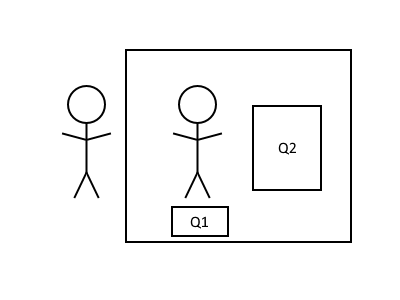
\includegraphics[width=0.5\textwidth]{a.png}}
%
%%%%%%
\ffigbox{\caption*{1.2: Wie das Problem fälschlicherweise gemessen wird}}%
{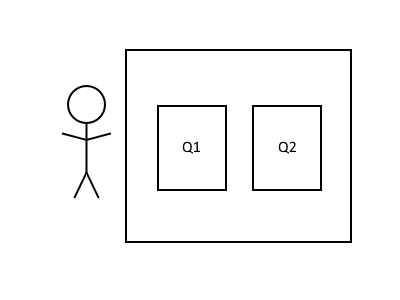
\includegraphics[width=0.5\textwidth]{b.png}}
\end{floatrow}
\end{figure}
Allerdings bedeutet dies auch im Allgemeinen, dass es komplexer als erwartet ist, Berechnungen von einem geschachtelten Quantensystem durchzuführen, da man für jeden Anteil der Superposition des äusseren Systems auch eine komplette Superposition des inneren Systems abspeichern muss. Die genaue Beschreibung lasse ich aber hier aus, um mich wieder dem eigentlichen Gedankenexperiment zu widmen.\\\\
Zuerst schlage ich aber noch eine Vereinfachung des Gedankenexperiments vor: Die Aufgaben von $W_1$ und $W_2$ lassen sich auf eine einzelne Person, $W$, übertragen, da sich $W_1$ und $W_2$ selber nicht in einer Superposition befinden und in der gleichen Umgebung sind. Dies wird auch in den Abbildungen so sein. Im Artikel wird das Modell ähnlich grafisch dargestellt wie in Abbildung 2.1. Messtechnisch gesehen ist es aber korrekter das Modell darzustellen wie in Abbildung 2.2. Mein Argument dafür ist folgendes: $F_1$ misst das Zufallsbit $Q_1$, und prepariert $Q_2$ entsprechend nach dem Ergebnis der Messung von $Q_1$, bevor $Q_2$ zu $F_2$ verschickt wird. Um aber das Qubit nach $F_2$ zu schicken, darf $F_2$ erst isoliert werden, wenn $F_2$ das Qubit empfangen hat. Da aus $W$'s Sicht das Ganze aber in einer Superposition geschehen muss, muss die Isolation von $F_2$ im Labor von $F_1$ stattfinden. Praktisch sähe dies so aus, dass $F_1$ das Qubit $Q_2$ zusammen mit $F_2$ in $F_1$'s Labor isoliert, und dass dann $F_2$ innerhalb der Isolation $Q_2$ misst. Anschaulicher lässt sich dies mit einem Quantencomputer darstellen: Man misst ein Quantenbit in einer Superposition, und übergibt das Resultat zusammen mit dem Programm(oder sonst das Programm dem Resultat anpassen), und der Quantencomputer führt in Isolation das Programm aus.

\begin{figure}[!htb]
\begin{floatrow}[2]\
\ffigbox{\caption*{2.1: Wie das Gedankenexperiment dargestellt wird}}%
{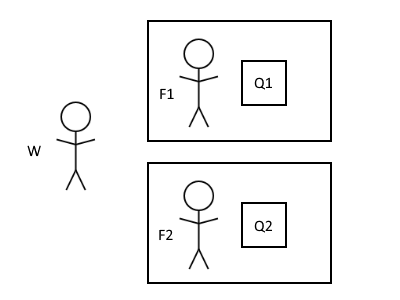
\includegraphics[width=0.5\textwidth]{c.png}}
%
%%%%%%
\ffigbox{\caption*{2.2: Wie das Gedankenexperiment logisch dargestellt werden sollte}}%
{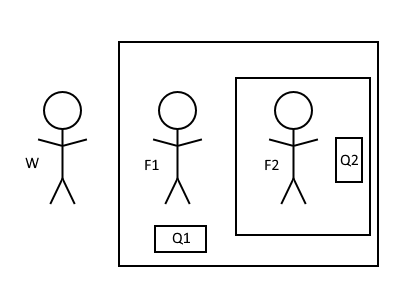
\includegraphics[width=0.5\textwidth]{d.png}}
\end{floatrow}
\end{figure}
Da wir nun das Modell geschachtelt dargestellt haben, können wir unsere Erkenntnis aus dem simpleren Problem darauf anwenden.

\end{document}